\chapter{Excitations and Defects in Quantum Materials}

Session 8 left us with a small zoo of freshly built ground states: quantum spin liquids described
by mean-field spinons, and Kondo lattices whose local moments, screened by conduction electrons
through the very same Abrikosov-fermion trick, turn a metal into a heavy-fermion insulator. Every
session up to this point has followed the same basic move: take a many-body Hamiltonian, find a
controlled or approximate reformulation, and read off the ground state that comes out. Today we do
something different with all of that machinery. Rather than building one more ground state, we are
going to \emph{probe} the ground states we already have. The idea is simple to state: take a quantum
material, metal, superconductor, topological insulator, quantum magnet, whichever one you like,
disturb it a little, and watch how it responds. It turns out that the response itself, computed
entirely from the undisturbed ground state, tells us an enormous amount about what that ground
state actually is. We will run this one idea, linear response, as a probe over essentially every
system class the course has built so far: ordinary metals, session 5's superconductors, sessions
3 and 4's topological matter, and session 8's quantum magnets, and in each case we will see the
response function acting as a diagnostic, reading off Fermi surfaces, superconducting pairing
symmetries, topological invariants, and spin gaps, all from the same underlying formalism. Along
the way we will also see the Stoner criterion for itinerant magnetism fall directly out of the
same response-function language, reconnecting to session 1 and session 6's magnetism, but now
viewed as an \emph{instability} of the paramagnetic response rather than as a mean-field ground-state
ansatz we imposed by hand. Today's session is, in that sense, the course's diagnostic and synthesis
session: less a new building block than a new lens trained on everything we have already built.

\section{Framing: response functions as a probe of the ground state}

Let us set up the general experiment we have in mind, because the same setup is going to recur in
every example today. We take a quantum material with some ground state we understand (or think we
understand), and we make a small perturbation at position $x$ and time $t$. Then we measure some
observable at a different position $x'$ and a different (typically later) time $t'$. The relation
between what we did at $(x,t)$ and what we observe at $(x',t')$ is encoded in a \textbf{response
function}, and once we know that function completely, we know how the material reacts to a
perturbation applied anywhere, at any time.

The power of this framing is that it is completely observable-agnostic. The same formalism covers:

\begin{itemize}
\item a perturbation in the local electrostatic potential, measured as a change in the local charge
  density, giving the \textbf{dielectric function};
\item a local magnetic moment or field, measured as a change in the local magnetization elsewhere,
  giving the \textbf{magnetic susceptibility} (equivalently, the spin-fluctuation response);
\item a local temperature change, measured as a change in temperature elsewhere, giving the
  \textbf{thermal conductance}.
\end{itemize}

There are also two quite different ways of actually running this experiment in the lab, and it is
worth having both in mind, because we will use each type of example today. One route is a genuine
physical perturbation: substitute one atom of a metal for a different element, and you have created
a real, localized impurity. As we will see in detail in Section 9.6, the resulting \textbf{Friedel
oscillations} in the electronic density directly reveal the material's Fermi surface. The other
route is that the measurement itself is the perturbation: fire a neutron, whose own magnetic
moment couples to the local moments in a magnetic material, and the scattering cross-section you
record is a direct readout of the material's magnetic fluctuations (inelastic neutron scattering).
These look like very different experiments, but the underlying formalism, and the kind of
information you extract, is the same in both cases.

Finally, a simplification that will make almost everything below tractable: whenever the
unperturbed Hamiltonian has translational symmetry in space and is time-independent, the response
function can only depend on $x'-x$ and $t'-t$, not on $x,t,x',t'$ separately. That is precisely
the situation in which Fourier transforming to reciprocal space and frequency, $(q,\omega)$, is the
natural language, and it is the language we will use for essentially the rest of this session.

\section{A classical warm-up: the response of a classical magnet}

Before bringing in any quantum many-body machinery, it is worth seeing the whole logic of ``response
predicts the ground state'' play out in a setting we already know how to solve exactly: a classical
Ising magnet at finite temperature, treated in mean-field theory (recall Section 1.12 for the
mean-field recipe itself). The question we want to ask is genuinely useful: sitting at a
temperature well above any ordering transition, is there a measurement we can make \emph{right there},
in the disordered phase, that tells us what kind of order the system is heading toward as we cool
it down?

The relevant response is the \textbf{magnetic susceptibility}, $\chi = \partial M/\partial H$, the
linear-response coefficient relating an applied field $H$ to the magnetization $M$ it induces.
Solving the mean-field Ising model at high temperature gives three distinct behaviors, depending
on the sign and strength of the exchange coupling:

\begin{equation}
\chi(T) \;\propto\;
\begin{cases}
\dfrac{1}{T} & \text{paramagnet (no exchange coupling), diverges only at } T=0, \\[4pt]
\dfrac{1}{T - T_c} & \text{ferromagnet, diverges at a positive } T_c, \\[4pt]
\dfrac{1}{T + T_c} & \text{antiferromagnet, apparent divergence at a negative temperature.}
\end{cases}
\end{equation}

The physical picture behind (9.1) is worth holding on to, because we are going to meet it again,
in a fully quantum guise, in Section 9.5. In the paramagnetic regime, thermal fluctuations dominate
and the susceptibility stays finite at any $T>0$: nothing is trying to order. In the ferromagnetic
case, fluctuations \emph{reinforce} the applied field, so as $T\to T_c^+$ the system polarizes more and
more easily, and $\chi$ genuinely diverges right at the transition. In the antiferromagnetic case,
fluctuations \emph{fight} the applied field (favoring staggered rather than uniform order), which shows
up as the opposite sign in the denominator: the susceptibility looks like it is heading toward a
divergence at a temperature below absolute zero, which of course it never reaches, but the sign
alone already tells you the ordering tendency is antiferromagnetic rather than ferromagnetic.
Experimentally, this is a genuinely practical diagnostic: plot $\chi^{-1}(T)$, and a straight line
extrapolating to a positive intercept signals an incipient ferromagnet, a negative intercept an
incipient antiferromagnet, all measured entirely from the disordered high-temperature phase. This
is the conceptual template for the entire session: \textbf{the response of the disordered/uniform state,
computed without ever solving for the ordered state itself, already contains the information about
which ordered state is coming.}

\section{Linear response and perturbation theory, done properly}

Let us now build the quantum version of this idea carefully, since everything that follows rests
on it. Split the full Hamiltonian into an unperturbed piece $H_0$ (a metal, a superconductor, a
quantum magnet, whatever system we are studying) and a perturbation $V$, with a bookkeeping
coupling constant $\lambda$ that we will eventually set to one:

\begin{equation}
H(\lambda) = H_0 + \lambda V, \qquad \lambda = 0 \;\text{(pristine)}, \quad \lambda = 1\;\text{(full perturbation)}.
\end{equation}

Every observable of the system, energies, densities, magnetizations, wavefunctions themselves,
becomes a function of $\lambda$ once we fix $H(\lambda)$. If that function is smooth enough to
Taylor-expand around $\lambda=0$ (we will come back to exactly when this assumption fails), then
for any observable $A$,

\begin{equation*}
A(\lambda) = A^{(0)} + \lambda\, \chi_A + O(\lambda^2), \qquad
\chi_A \equiv \left.\frac{\partial A}{\partial \lambda}\right|_{\lambda=0},
\end{equation*}

and by definition $\chi_A$, the first-order coefficient, \emph{is} the response function we have been
talking about all session. To actually compute $\chi_A$ for a generic observable, we first need
the perturbed wavefunctions. Expanding an unperturbed eigenstate $|n\rangle$ of $H_0$ (energy
$E_n^{(0)}$) in the full basis $\{|m\rangle\}$ of $H_0$, standard Rayleigh-Schrödinger perturbation
theory gives, to first order in $\lambda$ and away from any degeneracy,

\begin{equation}
|n(\lambda)\rangle = |n\rangle + \lambda \sum_{m \neq n} \frac{\langle m|V|n\rangle}{E_n^{(0)} - E_m^{(0)}} \, |m\rangle + O(\lambda^2).
\end{equation}

The structure of (9.3) is worth keeping firmly in view, because it is the engine behind every
derivation in the rest of this session: a perturbation mixes a state $|n\rangle$ with every other
state $|m\rangle$, weighted by the matrix element of $V$ between them, and suppressed by the inverse
energy gap between the two states. States close in energy mix strongly; states far apart barely
mix at all. Once we have (9.3), any observable, in particular any density or magnetization, can be
written down to first order in $\lambda$ by inserting the perturbed states.

\textbf{When does this break down?} The whole construction in (9.3) presupposes that $A(\lambda)$ is an
analytic function of $\lambda$ near $\lambda=0$, and that assumption is not automatic. Three
paradigmatic quantum states are known to be intrinsically non-perturbative in exactly this sense,
worth flagging explicitly since they mark the boundary of everything derived below:

\begin{itemize}
\item \textbf{An impurity in a metal, the orthogonality catastrophe.} In the thermodynamic limit, the full
  many-body wavefunction of a metal with an impurity switched on becomes exactly orthogonal to the
  wavefunction with the impurity switched off, no matter how weak the impurity potential is.
\item \textbf{A quantum spin in a metal, the Kondo effect.} The emergent Kondo temperature is a
  non-perturbative function of the Kondo coupling (it involves an essential singularity, not a
  power series, in the coupling constant).
\item \textbf{Superconductivity in the BCS limit.} The superconducting gap is likewise non-perturbative in
  the attractive coupling constant.
\end{itemize}

For the rest of this session we restrict ourselves to the regime where perturbation theory \emph{does}
hold, which is where (9.2) and (9.3) give a controlled, systematic way of computing responses.

\section{The Fermi sea and the Lindhard function}

To make (9.3) concrete, let us specialize to the case that will occupy most of today: a
non-interacting electronic Hamiltonian in diagonal form, $H_0 = \sum_k \varepsilon(k)\, c_k^\dagger
c_k$. Its many-body ground state is the Fermi sea: fill every single-particle state with
$\varepsilon(k)$ below the Fermi energy, leave every state above it empty. Correspondingly,
$\langle c_k^\dagger c_k\rangle = n_F(\varepsilon(k))$, equal to $1$ for occupied states and $0$ for
unoccupied ones (at $T=0$; more generally the Fermi-Dirac function), and the set of $k$-points
sitting exactly at the Fermi energy defines the \textbf{Fermi surface}. This surface is going to be the
single most important geometric object in everything that follows, because a small perturbation can
only rearrange states close to it: moving an electron from deep in the Fermi sea to deep above it
costs far too much energy to matter at first order.

Now apply (9.3) with a specific, physically motivated perturbation: a local shift of the on-site
energy, i.e. a local change in the chemical potential at one point in the material. The observable
we track is the change in local electronic density, $n(x) - n_0(x)$. Using translational symmetry,
Fourier transform to $q$-space and insert the perturbed wavefunctions (9.3) into the density
operator; after some algebra (each term comes from a matrix element $\langle k+q|V|k\rangle$
divided by the energy denominator $\varepsilon(k+q)-\varepsilon(k)$, exactly the structure of
(9.3)) one obtains the \textbf{static Lindhard function},

\begin{equation}
\chi_0(q) = \frac{1}{N} \sum_k \frac{n_F(\varepsilon(k)) - n_F(\varepsilon(k+q))}{\varepsilon(k+q) - \varepsilon(k)}.
\end{equation}

It is worth checking (9.4) makes sense before using it. As $q\to 0$, expanding both numerator and
denominator to first order in $q$ gives $\chi_0(q\to 0) \to -\sum_k n_F'(\varepsilon(k))/N$, which
at $T=0$ is exactly $D(E_F)$, the density of states per site at the Fermi level: a positive,
finite number, as it should be. Equation (9.4) is non-zero only when $k$ is occupied and $k+q$ is
unoccupied (or vice versa); if both are occupied or both empty, the numerator vanishes. So the
response is built entirely out of states straddling the Fermi surface, exactly as the general
argument above anticipated.

\textbf{Instabilities and nesting.} Equation (9.4) has a striking feature in one dimension. If there
exists a wavevector $q^\star$ connecting an occupied state at $k$ to an empty state at $k+q^\star$
of the \emph{same} energy, the denominator in (9.4) vanishes right at that term, and $\chi_0(q^\star)$
diverges. For a generic 1D band the Fermi surface is just the two points $\pm k_F$, and the single
nesting vector connecting them is $q^\star = 2k_F$ (figure~\ref{fig:s09:nesting}a,b); summing (9.4) over the whole band gives a
logarithmic divergence, $\chi_0(2k_F) \sim \ln(W/T)$ (with $W$ a bandwidth cutoff), which is exactly
the Peierls instability that drives one-dimensional metals to dimerize into a charge density wave.
Physically: a response function that diverges means an arbitrarily weak perturbation at that
wavevector produces an arbitrarily large rearrangement of the ground state, i.e. the ground state
we started from is unstable to that particular fluctuation. This is the central strategic idea we
will keep reusing: to predict a new phase of matter, look for the wavevector at which the response
function of the old phase diverges.

Everything above generalizes straightforwardly to finite frequency: repeating the derivation with a
time-dependent perturbation $\propto e^{-i\omega t}$ gives the (retarded) \textbf{dynamical Lindhard
function},

\begin{equation}
\chi_0(q,\omega) = \frac{1}{N} \sum_k \frac{n_F(\varepsilon(k)) - n_F(\varepsilon(k+q))}{\varepsilon(k+q) - \varepsilon(k) - \hbar\omega - i0^+},
\end{equation}

which reduces to (9.4) at $\omega = 0$. For a one-dimensional chain, plotting $\mathrm{Im}\,\chi_0(q,\omega)$
over the whole $(q,\omega)$ plane produces a characteristic surface of divergences that traces out
the particle-hole continuum of the band structure; this $\omega$-$q$ plot is slide-only material,
the spoken lecture describes its shape in words (``a whole collection of $\omega$ versus $q$ values
where there are divergences'') but never draws it, so the figure itself is worth opening the slides
for.

The same logic extends cleanly to two dimensions. For a square lattice with dispersion
$\varepsilon(k) = -2t(\cos k_x + \cos k_y)$, low filling gives a small, roughly circular Fermi
surface, and $\chi_0(q,0)$ is correspondingly large for $q$ inside a circle set by the
Fermi surface's diameter and small outside it: the response function is, quite literally, a picture
of the Fermi surface. This is the physical basis of \textbf{quasiparticle interference (QPI)}: real STM
experiments put impurities into a 2D metal, image the resulting modulation of the local density of
states, and invert the observed wavelength to read off the Fermi surface. At half filling, however,
the square lattice's particular dispersion gives $\varepsilon(k+Q) = -\varepsilon(k)$ for
$Q=(\pi,\pi)$: a \emph{perfect} nesting condition connecting enormous portions of the Fermi surface
(which is itself a square of straight lines at half filling, not a circle) all at the same
wavevector simultaneously. Equation (9.4) then develops a massive divergence exactly at
$q=(\pi,\pi)$, signaling a strong instability there. Figure~\ref{fig:s09:nesting} collects the whole
argument in one place: the single 1D nesting vector, the logarithmic divergence it produces in
$\chi_0(q)$, and the straight-edged 2D Fermi surface that $Q=(\pi,\pi)$ nests all at once. The
half-filling Fermi surface shape and the
explicit nesting vector are shown on the slides more concretely than described in speech; it is
worth looking at that figure directly to see the straight parallel edges that make the
$(\pi,\pi)$ nesting so effective.

% Session 9 -- Fermi-surface nesting: where the Lindhard function diverges.
% Placement: sec. "The Fermi sea and the Lindhard function", at the
% Rendered by figures/blender/s09f01_nesting.py, labels in figures/overlays/s09f01_nesting.tex.
\begin{aqmfigure}{fig:s09:nesting}{Nesting is what makes a response function diverge. (a) A
one-dimensional band $\varepsilon(k)=-2t\cos k$ at partial filling. The occupied states (thick) end
at $\pm k_F$, and the single wavevector $q^\star=2k_F$ connects one Fermi point to the other, so the
energy denominator of (9.4) vanishes for that term. (b) The static Lindhard function that results,
with the closed form given in Section 9.6. It is finite and equal to $D(E_F)$ as $q\to0$, as the
$q\to0$ check of (9.4) requires, and it diverges logarithmically at $q^\star=2k_F$, which is the
Peierls instability. (c) In two dimensions the criterion becomes geometric. At half filling the
Fermi surface of the square lattice is the diamond with straight edges $|k_x|+|k_y|=\pi$, and since
$\varepsilon(k+Q)=-\varepsilon(k)$ for $Q=(\pi,\pi)$, this one vector, the red arrows, maps
\emph{every} point of one edge onto the parallel opposite edge at the same time. For this reason the
divergence at $(\pi,\pi)$ is much stronger than the one-dimensional one, since whole segments of the
Fermi surface nest, and not isolated points. At low filling the same Fermi surface is a small
circle, which no single $q$ can nest in this way.}
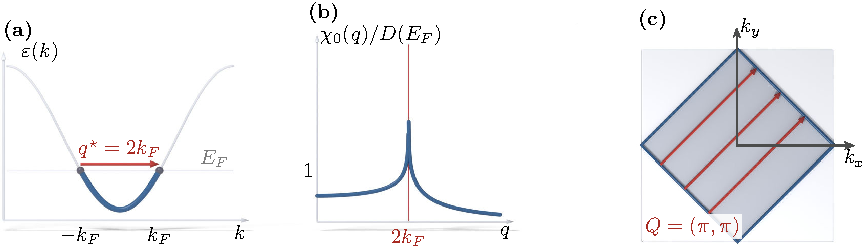
\includegraphics{figures/pdf/s09f01_nesting.pdf}
\end{aqmfigure}


\begin{notebookbox}{\texttt{session9.ipynb}, ``The charge-charge response function'' (Challenge)}
Plot $\mathrm{Im}\,\chi_0(q,\omega)$ for a tunable band structure and chemical potential $\mu$,
exactly as in (9.5). Watch the divergence track the Fermi surface as you change $\mu$, and see
whether you can predict, from the band structure alone, which $q$-vector the instability will sit
at, before running the calculation.
\end{notebookbox}

\section{Interactions as a perturbation: RPA, plasmons, and the Stoner instability}

So far the perturbation has been an external impurity. Nothing stops us from treating the
electron-electron interaction \emph{itself} as the perturbation, using $\chi_0$, the non-interacting
response we just built, as input, and asking for the response $\chi$ of the full interacting
system. We need two things: a rule connecting $\chi$ to $\chi_0$, and a criterion for reading
instabilities off of $\chi$.

\textbf{From $\chi_0$ to $\chi$: the random phase approximation.} Consider a contact (Hubbard-like)
interaction of strength $U$ coupling to the density. The physical picture is a diagrammatic one:
the response to a probe is the bare response $\chi_0$, plus the bare response followed by one
interaction event and another bare response, plus two interaction events, and so on, an infinite
ladder of terms. This is most efficiently captured not by summing the series term by term but by
writing down the self-consistent equation the full response must satisfy,

\begin{equation*}
\chi(q,\omega) = \chi_0(q,\omega) + \chi_0(q,\omega)\, U\, \chi(q,\omega),
\end{equation*}

which solves algebraically to give the \textbf{random phase approximation (RPA)},

\begin{equation}
\chi(q,\omega) = \frac{\chi_0(q,\omega)}{1 - U\,\chi_0(q,\omega)}.
\end{equation}

Equation (9.6) is a curious hybrid: derived order by order in $U$, it is perturbative, but the act
of resumming the whole geometric series makes it non-perturbative, capturing physics (a genuine
pole, i.e. a genuine phase transition) that no finite order in $U$ alone ever could.

\textbf{Two distinct sources of divergence.} The interacting response (9.6) can diverge for two quite
different reasons, and it is worth telling them apart because they correspond to two different
emergent quasiparticles.

\emph{From $\chi_0$ itself}, exactly as in Section 9.4: an electron-hole excitation, a single-particle
process, moving one electron from an occupied to an empty state.

\emph{From the RPA denominator}, $1-U\chi_0=0$, which is a genuinely new, collective phenomenon coming
from the interaction. For a long-range Coulomb interaction, $U \to v(q)$, with a strong $q$-dependence
(diverging as $q\to0$), the pole of (9.6) as a function of $\omega$ at fixed $q$ defines a new
quasiparticle, the \textbf{plasmon}: a collective charge oscillation of the whole electron gas. Its
dispersion depends on the screening and dimensionality of the system, but in the standard RPA
(Bohm-Pines) treatment of the three-dimensional electron gas, at long wavelength it takes the form

\begin{equation}
\omega_{\rm pl}(q)^2 = \omega_p^2 + \tfrac{3}{5} v_F^2\, q^2 + O(q^4),
\end{equation}

with $\omega_p$ the classical plasma frequency; the plasmon survives even at $q=0$, unlike the
particle-hole continuum, because it is a genuinely collective mode of the whole charge density
rather than a single-particle excitation. Figure~\ref{fig:s09:plasmon} puts both kinds of divergence
on the same $(q,\omega)$ plane, and shows explicitly the small-$q$ window in which the pole exists
and no single-particle excitation does.

% Session 9 -- the two sources of divergence in the RPA response: the
% particle-hole continuum inside chi_0, and the collective plasmon pole of the
% RPA denominator.
% Placement: sec. "Interactions as a perturbation", after equation (9.7).
\begin{aqmfigure}{fig:s09:plasmon}{The two divergences of the RPA response (9.6), drawn in the
$(q,\omega)$ plane for the three-dimensional electron gas. The shaded region is where
$\mathrm{Im}\,\chi_0(q,\omega)\neq0$, which is the \emph{particle-hole continuum}, the set of all
$(q,\omega)$ at which a single electron can be moved from an occupied state $k$ to an empty state
$k+q$. Its upper boundary is $\hbar\omega_+=\hbar v_Fq+\hbar^2q^2/2m$, and beyond $2k_F$ a lower
boundary $\hbar\omega_-=\hbar^2q^2/2m-\hbar v_Fq$ appears. Both follow from the energy denominator of
(9.5), and for $q<2k_F$ the continuum goes all the way down to $\omega=0$, which is the same statement
as saying that $\chi_0$ is built only from states on the two sides of the Fermi surface. The plasmon
(9.7) is a different object. It is a zero of the RPA \emph{denominator} $1-v(q)\chi_0$, so it exists
at $\omega_p$ even as $q\to0$, in a window where no single-particle excitation exists at all. This
window, marked in the figure, is the full meaning of the phrase ``collective mode, not a
particle-hole pair''. Once the branch meets the continuum it can decay into particle-hole pairs, and
it is Landau damped (dashed).}

\begin{tikzpicture}
\begin{axis}[
  aqmplot,
  width=10.8cm, height=6.4cm,
  axis lines=left,
  axis line style={aqm, black},
  xlabel={$q$}, ylabel={},
  xmin=0, xmax=2.30, ymin=0, ymax=5.35,
  xtick={2}, xticklabels={$2k_F$},
  ytick={1.3}, yticklabels={$\omega_p$},
  xlabel style={at={(axis description cs:1.0,-0.02)}, anchor=north east},
  enlargelimits=false,
]

% --- the particle-hole continuum -------------------------------------------
% fill everything under omega_+ = v_F q + hbar q^2 / 2m ...
\addplot[draw=none, fill=aqmfill, domain=0:2.28, samples=90] {x + x^2/2} \closedcycle;
% ... then cut the region below omega_- back out again, for q > 2 k_F
\addplot[draw=none, fill=white, domain=2:2.28, samples=30] {x^2/2 - x} \closedcycle;
% boundaries
\addplot[aqmmuted, solid, line width=0.8pt, smooth, domain=0:2.28, samples=90] {x + x^2/2};
\addplot[aqmmuted, solid, line width=0.8pt, smooth, domain=2:2.28, samples=30] {x^2/2 - x};

\node[aqmlabsmall, anchor=south east, text=aqmmuted] at (axis cs:2.28,4.40) {$\omega_+$};
\node[aqmlabsmall, anchor=south east, text=aqmmuted] at (axis cs:2.29,0.40) {$\omega_-$};

\node[aqmlab, anchor=center, align=center, text width=4.2cm] at (axis cs:1.64,0.74)
  {\textbf{particle-hole continuum}\\[1pt]
   \footnotesize $\mathrm{Im}\,\chi_0\neq0$: one electron, one hole};

% --- the plasmon branch ------------------------------------------------------
% omega_pl = sqrt(omega_p^2 + (3/5) v_F^2 q^2), undamped until it meets omega_+
\addplot[aqmcurve, line width=1.5pt, domain=0:1.01, samples=50] {sqrt(1.69 + 0.6*x^2)};
\addplot[aqmaccent, smooth, line width=1.2pt, dash pattern=on 3.5pt off 2pt,
         domain=1.01:2.28, samples=60] {sqrt(1.69 + 0.6*x^2)};
\node[circle, draw=aqmaccent, fill=aqmaccent, minimum size=4.5pt, inner sep=0pt]
  at (axis cs:0,1.3) {};

% --- annotations, all kept in the empty upper-left quadrant ------------------
\node[aqmlabsmall, anchor=north west, align=left, text=aqmaccent, text width=3.4cm]
  at (axis cs:0.06,5.28)
  {\textbf{plasmon}: a zero of the RPA denominator $1-v(q)\chi_0$, collective};
\draw[aqmarrowaccent, line width=0.6pt] (axis cs:0.94,4.30) -- (axis cs:0.86,1.50);

\node[aqmlabsmall, anchor=north west, align=left, text=aqmbroken, text width=3.4cm]
  at (axis cs:0.06,3.68)
  {no particle-hole excitation exists in this window --- and yet the response has a pole};
\draw[aqmarrowbroken, line width=0.6pt, dash pattern=on 2pt off 1.5pt]
  (axis cs:0.30,2.62) -- (axis cs:0.28,1.46);
\draw[aqm, draw=aqmbroken, {Stealth[length=4pt,width=3.2pt]}-{Stealth[length=4pt,width=3.2pt]}]
  (axis cs:0.28,0.34) -- (axis cs:0.28,1.29);

\node[aqmlabsmall, anchor=south east, align=right, text=aqmbroken, text width=2.6cm]
  at (axis cs:2.28,2.25) {meets the continuum:\\[-1pt]Landau damped};

\node[aqmlabsmall, anchor=south] at (axis cs:0,5.42) {$\omega$};

\end{axis}
\end{tikzpicture}

\end{aqmfigure}


\textbf{The Stoner criterion, as a response-function instability.} Now apply the same RPA logic to the
\emph{spin} channel of a Hubbard-type interaction, so $\chi_0$ in (9.6) becomes the non-interacting spin
susceptibility. The interacting spin response diverges precisely when

\begin{equation}
U\, \chi_0(q,0) = 1.
\end{equation}

At $q=0$, using the $q\to0$ limit of (9.4), $\chi_0(0,0) = D(E_F)$, so (9.8) reduces to
$U\,D(E_F) = 1$: this is exactly the \textbf{Stoner criterion} for itinerant ferromagnetism, an
interacting metal becomes magnetic once the product of the density of states at the Fermi level and
the interaction strength crosses one. But (9.8) is more general than the $q=0$ special case: for a
Fermi surface with strong nesting, such as the half-filled square lattice of Section 9.4,
$\chi_0(q,0)$ is \emph{maximized} not at $q=0$ but at the nesting vector $Q=(\pi,\pi)$, where it is
already logarithmically enhanced. The instability threshold in (9.8) is then reached first at
$Q=(\pi,\pi)$ rather than at $q=0$: the system develops a \emph{staggered}, antiferromagnetic instability
rather than a uniform ferromagnetic one, at a smaller value of $U$ than the naive Stoner estimate
would suggest.

It is worth pausing on this, because it is exactly the reconnection the course has been building
toward. Sessions 1 and 6 derived magnetism by writing down the Hubbard model, applying mean-field
theory directly to the \emph{ordered} state, and self-consistently solving for a non-zero magnetization
$m$ (Section 1.13's Equation 1.7). Today we have derived the \emph{same physics}, the same threshold
$U\,D(E_F)=1$, the same preference for antiferromagnetism at half filling, without ever writing
down an ordered mean-field ansatz: we asked instead when the \emph{paramagnetic}, disordered response
function develops a divergence, exactly the same logic as Section 9.2's classical susceptibility.
Mean-field theory and the response-function view are two routes to the same instability, one
computed from the broken-symmetry side, one computed entirely from the symmetric side by watching
it become unstable.

The same machinery, applied to different response channels and different signs of interaction,
classifies a whole family of instabilities that is worth laying out explicitly (this three-way
classification is presented as a clean summary table on the slides, more systematically than the
spoken walkthrough, which mainly worked the magnetic case through in detail):

\begin{center}
\begin{tabular}{lll}
\hline
Instability & Response channel & Interaction sign \\
\hline
Magnetism & spin response & repulsive \\
Dimerization / charge density wave & charge-phonon response & repulsive \\
Superconductivity & electron-electron scattering response & attractive \\
\hline
\end{tabular}
\end{center}

\begin{notebookbox}{\texttt{session9.ipynb}, ``The charge-charge response function'' (Challenge)}
The same notebook section used above for nesting extends, in its second part, to the interacting
case: add a Hubbard interaction $U$ and an external staggered (antiferromagnetic) field to a
dimerized chain, and watch what happens to the response as $U$ increases. This is the
notebook-scale version of equation (9.8), the Stoner instability appearing as $U$ crosses the
threshold set by $\chi_0$.
\end{notebookbox}

\section{Impurities as diagnostics I: Friedel oscillations in a metal}

We now turn to the most physical realization of a perturbation: an actual local impurity. Four
case studies follow, one for each broad class of ground state we have built over the course:
metals, superconductors, topological matter, and quantum magnets. In each case the diagnostic logic
is the same: perturb locally, and read the nature of the ground state off of how the perturbation's
effect decays in space.

Start with a metal. An impurity is a local on-site energy shift, and adding one to a translationally
symmetric Hamiltonian necessarily breaks that symmetry, but note that perturbation theory itself
never required translational symmetry in the first place: equations (9.2) and (9.3) hold for any
$H_0$ and any $V$. Applying them directly to the local density of states gives a response
proportional to matrix elements between Fermi-surface states, and for a generic (parabolic-like)
band the resulting oscillation is set entirely by the Fermi wavevector.

To see this rigorously, note that the static Lindhard function of a one-dimensional free-electron
gas has the closed form

\begin{equation*}
\chi_0(q) = \frac{m}{\pi\hbar^2 q}\ln\left|\frac{2k_F + q}{2k_F - q}\right|,
\end{equation*}

which is smooth everywhere except for a logarithmic non-analyticity exactly at $q = 2k_F$, the very
same nesting singularity identified in Section 9.4. A standard fact of Fourier analysis is that a
non-analyticity of a function $\chi_0(q)$ at a wavevector $q^\star$ produces an algebraically
decaying oscillatory tail in its real-space Fourier transform, with period fixed by $q^\star$ and
an envelope set by the \emph{type} of the singularity. Applying this to the impurity-induced density
change $\delta n(x) = \int \frac{dq}{2\pi}\, e^{iqx}\, \chi_0(q)\, v_0$ (Born approximation, impurity
strength $v_0$) gives the \textbf{Friedel oscillation},

\begin{equation}
\delta n(x) \;\xrightarrow{|x|\to\infty}\; A(v_0)\, \frac{\cos\!\big(2k_F |x| + \varphi_0\big)}{|x|^{\,d}} \qquad (d = 1,2,3),
\end{equation}

with a universal oscillation wavevector fixed purely by the Fermi surface ($2k_F$ in 1D, or the
Fermi-surface diameter more generally), an algebraic envelope whose power depends on the
dimensionality $d$, and a non-universal amplitude and phase set by the impurity strength and
microscopic details. This is a genuinely elegant closure of the loop opened in Section 9.4: the
very same $q=2k_F$ singularity in $\chi_0(q)$ that we identified there as an instability channel is,
here, what produces a long-ranged, power-law-decaying real-space oscillation, rather than an actual
instability, because a single local impurity is far too weak a perturbation to reorganize the whole
Fermi sea; the divergence in $\chi_0(q)$ just makes its Fourier partner decay slowly rather than
exponentially.

Concretely, for a one-dimensional tight-binding chain with an impurity at site $0$, the local
density of states oscillates around the impurity with wavelength $\pi/k_F$ (half the Fermi
wavelength $\lambda_F=2\pi/k_F$, since the modulation is set by $2k_F$ rather than by $k_F$), and
raising the chemical potential shortens $k_F^{-1}$ and speeds up the oscillation
correspondingly; the same phenomenon appears, with the same physical content, in a two-dimensional
square lattice, and this real-space LDOS modulation around impurities is exactly what an STM
measures in practice (this is quasiparticle interference again, seen this time in real rather than
reciprocal space). The explicit LDOS-versus-position plots at two different fillings, for both the
1D and the 2D case, are genuinely clearer on the slides than in words: the ``oscillations get faster
as $k_F$ grows'' comparison is a visual one, worth looking at directly rather than only reading the
formula. As a complementary check, the slides (and notebook) also show the \emph{insulating} case: an
impurity placed in a gapped 1D chain produces an LDOS that converges to its uniform value very
quickly rather than oscillating with a slow power-law envelope, a preview of the gapped-versus-gapless
diagnostic that we will make fully general in Section 9.9 and draw in figure~\ref{fig:s09:decay}.

\begin{notebookbox}{\texttt{session9.ipynb}, ``Impurity in a 1d metal'' (Core), ``Impurities in a 2d metal'' (Core), and ``Impurity in an electronic insulator'' (Core)}
Place a single impurity in a 1D chain, then a 2D square lattice, and watch the LDOS oscillate as
in (9.9). Change the chemical potential and confirm that the oscillation wavelength tracks
$\pi/k_F$ exactly as predicted; this is the cleanest place in the whole session to see a response
formula and a numerical experiment agree digit for digit. The third section repeats the exercise
with the chemical potential inside a gap instead of a partially filled band: confirm that the LDOS
now converges to its bulk value within a site or two, with no slowly-decaying oscillatory tail,
exactly the gapped-versus-gapless contrast that Section 9.9 makes fully general.
\end{notebookbox}

\section{Impurities as diagnostics II: magnetic impurities in a superconductor}

Superconductors behave completely differently under a local perturbation, because a superconductor
is, for single-particle excitations, a bulk insulator: there is a finite gap $\Delta$, so there is
no Fermi surface to produce Friedel-type oscillations. The interesting physics instead concerns the
distinction between magnetic and non-magnetic impurities.

Recall that an s-wave Cooper pair binds one spin-up and one spin-down electron. A \textbf{non-magnetic}
impurity, an ordinary local potential, does not distinguish spin up from spin down: it does not
break time-reversal symmetry, and so it cannot lower the energy cost of breaking any particular
Cooper pair. Concretely, the density of states of a conventional s-wave superconductor with and
without a non-magnetic impurity is essentially unchanged, gap and all: the slides show the two
spectra directly overlapping.

A \textbf{magnetic} impurity is entirely different: it couples with strength $J$ to the local spin,
distinguishes up from down, and therefore \emph{does} break time-reversal symmetry. This lowers the
energy cost of breaking one specific Cooper pair and produces a genuine bound state inside the gap.
In the classical-spin (Born) approximation this is the \textbf{Yu-Shiba-Rusinov} problem (the transcript
does not name it, but the setup matches it exactly): with $\alpha \equiv \pi
\nu_0 J S$ (where $\nu_0$ is the normal-state density of states at the Fermi level and $S$ the
impurity spin), the in-gap bound state energy is

\begin{equation}
E_b(J) = \Delta\, \frac{1-\alpha^2}{1+\alpha^2}.
\end{equation}

Equation (9.10) reproduces exactly the qualitative curve the slides show as a function of $J$: at
$J=0$ ($\alpha=0$), $E_b = \Delta$, sitting right at the gap edge, i.e. no genuine bound state yet.
As $J$ increases, $\alpha$ grows, and $E_b$ moves down through the gap; at $\alpha = 1$ (i.e.
$\pi\nu_0 J S = 1$) the state crosses zero energy exactly, and for $\alpha>1$ the numerator of
(9.10) turns negative, so the bound state re-emerges on the opposite side of zero. This crossing is
a genuine quantum phase transition: below it the many-body ground state has total spin $S_{\rm
tot}=0$ (every Cooper pair intact, the impurity spin screened into the condensate), above it
$S_{\rm tot}=1/2$ (one Cooper pair broken, leaving a single dangling spin). A superconductor with a
single, tunable magnetic impurity is therefore a minimal, exactly solvable model of a quantum phase
transition, driven entirely by a local perturbation. Both halves of the story are drawn in
figure~\ref{fig:s09:ysr}: the in-gap states that a magnetic impurity adds to an otherwise untouched
BCS spectrum, and the trajectory (9.10) traces across the gap as $\alpha$ grows.

% Session 9 -- Yu-Shiba-Rusinov states: what a magnetic impurity does to a
% Placement: sec. "Impurities as diagnostics II", after equation (9.10).
% Rendered by figures/blender/s09f03_ysr.py, labels in figures/overlays/s09f03_ysr.tex.
\begin{aqmfigure}{fig:s09:ysr}{A magnetic impurity in an s-wave superconductor. (a) The
single-particle density of states. The BCS continuum, with a gap $\Delta$ and coherence peaks at the
gap edges, is almost unchanged by a \emph{non-magnetic} impurity. Such an impurity does not
distinguish up from down, so it cannot lower the energy needed to break any specific Cooper pair. A
\emph{magnetic} impurity distinguishes them, breaks time-reversal symmetry, and creates a pair of
bound states inside the gap at $\pm E_b$, the red peaks, drawn for $\alpha=0.6$. (b) The energy of
these states, from (9.10), as a function of $\alpha=\pi\nu_0JS$. At $\alpha=0$ they are exactly at
the gap edges, meaning that there is no bound state yet. As the exchange grows they move across the
gap and cross at $\alpha=1$. The crossing is not a level repulsion that did not open. It is a real
quantum phase transition of the electronic ground state, with a change of fermion parity, and the
electron spin goes from $S_{\rm tot}=0$, where every Cooper pair is intact and the impurity spin is
not screened, to $S_{\rm tot}=1/2$, where one quasiparticle is bound to the impurity and partially
screens its spin. So a single impurity that we can tune is an exactly solvable quantum phase
transition.}
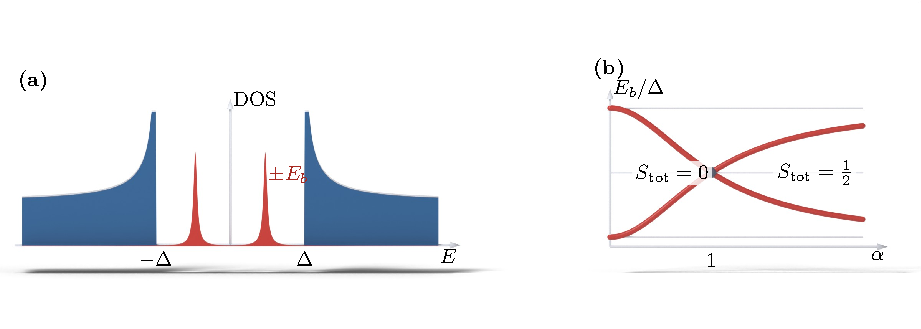
\includegraphics{figures/pdf/s09f03_ysr.pdf}
\end{aqmfigure}


\begin{notebookbox}{\texttt{session9.ipynb}, ``Magnetic impurities in a conventional superconductor'' (Core) and ``Single magnetic impurity in a superconductor'' (Challenge)}
Build a 1D superconducting chain with a magnetic impurity of tunable exchange $J$ and track the
in-gap state's energy exactly as in (9.10). Confirm the sign change at the crossing, and check
that a non-magnetic impurity (set $J=0$, vary only the local potential) leaves the gap edges
essentially untouched, as the qualitative argument above predicts.
\end{notebookbox}

\section{Impurities as diagnostics III: vacancies in topological matter}

The strongest possible local impurity is a \textbf{vacancy}: remove a site entirely, equivalently send
its on-site potential to infinity. This is where the bulk-boundary correspondence built in sessions
3 and 4 (Chern number, Zak phase, and the guarantee of gapless modes at any boundary of a
topologically non-trivial phase) pays off directly. Topological boundary modes are known to survive
around a large hole cut into a topological material; shrink that hole all the way down to a single
missing site, and the argument does not stop working. A vacancy is, in effect, a boundary of zero
size, and bulk-boundary correspondence still applies: whenever the bulk carries a non-trivial
topological invariant, a vacancy is guaranteed to host an in-gap bound state, as long as the vacancy
itself preserves the symmetry protecting that invariant.

This gives a genuinely useful diagnostic, because a fully gapped bulk spectrum on its own cannot
distinguish a topological phase from a trivial one. Take a \textbf{chiral, spin-triplet topological
superconductor} (the class studied via Majorana modes and Chern-number classification in session
5): its bulk spectrum, with no impurities, is fully gapped and looks, on its own, indistinguishable
from a trivial s-wave superconductor. But a vacancy is a non-magnetic perturbation (it does not
distinguish spin, so it preserves time-reversal symmetry, even in the extreme limit where the local
potential diverges), and once it is inserted, an in-gap mode appears. The same logic runs for a
\textbf{Chern insulator}: a vacancy in a system with finite Chern number produces an in-gap mode, while
the same vacancy in a topologically trivial insulator produces nothing of the sort. In both cases,
the observable signature is identical and simple: \emph{if introducing vacancies produces in-gap modes,
the underlying phase is topological; if it does not, the phase is trivial}, regardless of what the
clean bulk spectrum alone would have told you. Figure~\ref{fig:s09:vacancy} draws both the geometric
argument (a hole shrunk down to a single site) and the three spectra that make the diagnostic
usable.

% Session 9 -- a vacancy as a boundary of zero size, and why that makes it a
% Placement: sec. "Impurities as diagnostics III", after the bulk-boundary paragraph.
% Rendered by figures/blender/s09f04_vacancy.py, labels in figures/overlays/s09f04_vacancy.tex.
\begin{aqmfigure}{fig:s09:vacancy}{Why a single missing atom detects topology. Top, seen from above.
If we cut a large hole into a topologically non-trivial insulator or superconductor, the
bulk-boundary correspondence guarantees gapless modes that run around its edge. Nothing in that
argument depends on the size of the hole, so making it smaller does not remove these modes. A
vacancy is a boundary of zero size, and it binds an in-gap mode. Bottom, schematic spectra. This is
the diagnostic that a clean spectrum cannot give. A trivial and a topological insulator with the
same gap have bulk spectra that look the same, so nothing there distinguishes them (left). If we add
a vacancy, the trivial spectrum stays as it was (middle), and only the topological one develops a
state inside the gap (right). The rule is as direct as it looks. Vacancies produce in-gap modes if
and only if the bulk invariant is non-zero, provided that the vacancy itself respects the symmetry
that protects that invariant.}
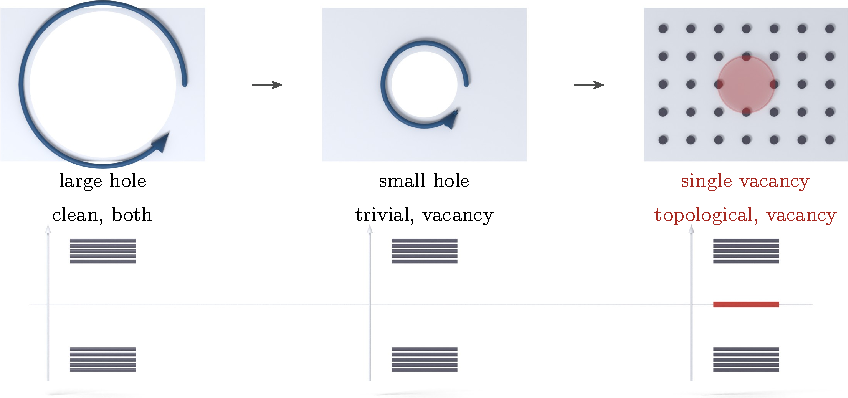
\includegraphics{figures/pdf/s09f04_vacancy.pdf}
\end{aqmfigure}


\begin{notebookbox}{\texttt{session9.ipynb}, ``Non-magnetic impurities in a topological superconductor'' (Challenge), ``DOS of non-magnetic impurities in a topological superconductor'' (Challenge), ``Single vacancy in a topological superconductor'' (Challenge), ``Vacancies in a topological insulator'' (Challenge), and ``Single vacancy in a topological insulator'' (Challenge)}
Build a chiral p-wave superconductor and a Chern (Haldane-model) insulator, each with a single
vacancy, and confirm the in-gap mode appears in both. The notebook's own suggested check is a
good one: swap the pairing symmetry to conventional s-wave, or the topological gap to a trivial
sublattice-imbalance gap, and watch the in-gap mode disappear, precisely because the bulk
invariant that guaranteed it via bulk-boundary correspondence is now zero.
\end{notebookbox}

\section{Impurities as diagnostics IV: screening in quantum magnets}

The last case study returns us to session 8's construction directly. Take a frustrated Heisenberg
model realizing a quantum-spin-liquid-like ground state: zero net magnetization on every site, and,
crucially, a ground state that does not break time-reversal symmetry. Add one local magnetic
perturbation and ask how the surrounding spins screen it.

For $S=1/2$, we do not need to redo the construction from scratch, session 8 already built exactly
the tool we need: represent each spin by a pair of auxiliary (Abrikosov) fermions, $S_i =
\tfrac{1}{2}\sum_{\alpha\beta} f_{i\alpha}^\dagger \boldsymbol{\sigma}_{\alpha\beta} f_{i\beta}$,
subject to the single-occupancy constraint $\sum_\sigma f_{i\sigma}^\dagger f_{i\sigma} = 1$ at every
site, and mean-field decouple the resulting quartic Hamiltonian. As derived in session 8, this turns
the Heisenberg model plus a local magnetic perturbation into a bilinear, tight-binding-like
Hamiltonian for the spinons, with an effective on-site term at the impurity site that mixes with the
spinon band. We are not going to re-derive that mapping here; see session 8's notes (its Abrikosov-fermion
construction) for the full mean-field decoupling.

What matters for us today is what this mapping buys us: it turns the ``screen a magnetic moment
embedded in a quantum spin liquid'' problem into \emph{exactly} the same mathematical problem as Section
9.6's ``impurity in a one-dimensional electron gas,'' just with electrons relabeled as spinons. The
induced spin correlation $\langle S_0 \cdot S_n\rangle$ as a function of distance $n$ from the
impurity therefore inherits the same structure as (9.9): an oscillation set by the antiferromagnetic
exchange, decaying with distance according to whether the underlying spinon band is gapped or
gapless.

This is where the comparison between $S=1/2$ and $S=1$ Heisenberg chains becomes sharp. Both realize
a spin-liquid-like ground state with zero on-site magnetization in the absence of an impurity, and
both develop an oscillating induced moment once the impurity is switched on, but the decay is
qualitatively different:

\begin{equation}
\langle S_0 \cdot S_n \rangle \;\sim\;
\begin{cases}
\dfrac{(-1)^n}{n} & S = 1/2 \quad \text{(power-law, gapless)}, \\[6pt]
(-1)^n\, e^{-n/\xi} & S = 1 \quad \text{(exponential, gapped)}.
\end{cases}
\end{equation}

The reason is exactly the reasoning behind (9.9) once more: the spin-$1/2$ Heisenberg chain maps, via
the Abrikosov-fermion construction, onto a gapless spinon tight-binding chain, with a genuine Fermi
surface (two points, as in Section 9.4's 1D metal), so the impurity response has to decay
algebraically, precisely as a metal's Friedel oscillations do. The spin-1 chain, in contrast, has an
excitation gap (the Haldane gap, not named explicitly in the transcript but exactly what opens for
integer-spin antiferromagnetic chains), which sets a finite correlation length $\xi$ and forces the
impurity response to decay exponentially, exactly as charge screening does inside a band insulator.

This gives us a completely general diagnostic, one that ties together every case study in this
session: \emph{power-law decay of an impurity response signals a gapless ground state; exponential decay
signals a gapped one, and the exponential's prefactor is literally the correlation length.} Section
9.6's metal (power law), the insulating chain noted at the end of that section (exponential), and
the two quantum-magnet cases here are all instances of the same underlying statement, drawn side by
side in figure~\ref{fig:s09:decay}.

% Session 9 -- the session's general diagnostic: power-law decay means gapless,
% Placement: sec. "Impurities as diagnostics IV", after equation (9.11).
% Rendered by figures/blender/s09f05_decay.py, labels in figures/overlays/s09f05_decay.tex.
\begin{aqmfigure}{fig:s09:decay}{The diagnostic that connects the whole session, drawn for the two
Heisenberg chains of (9.11). Close to the impurity both look the same, with an induced moment that
changes sign from site to site, because the exchange is antiferromagnetic. The only difference
between them is how the envelope decays. (a) The $S=1/2$ chain maps, through the Abrikosov-fermion
construction of session 8, onto a \emph{gapless} spinon band with a real Fermi surface of two
points, so its envelope decays as the power law $1/n$. This is the same mathematics, and the same
reason, as for the Friedel oscillations (9.9) of a metal. (b) The $S=1$ chain has the Haldane gap,
which fixes a finite correlation length $\xi$ and gives an exponential envelope $e^{-n/\xi}$, drawn
for $\xi=2.5$, in the same way as charge screening decays inside a band insulator. (c) On a
logarithmic vertical scale the two are easy to distinguish, since an exponential is a straight line
of slope $-1/\xi$ and a power law is not. The statement can be read in both directions, so a
measured decay law is a measurement of whether the ground state is gapped.}
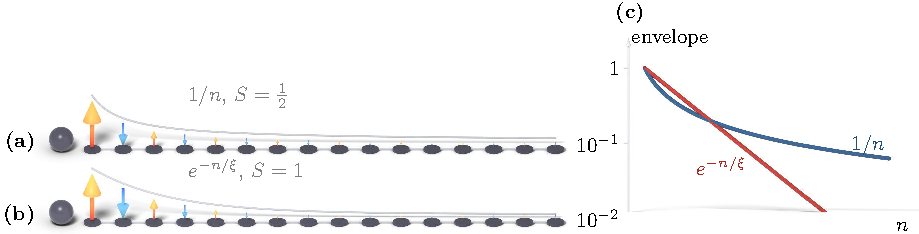
\includegraphics{figures/pdf/s09f05_decay.pdf}
\end{aqmfigure}


This particular sub-topic, screening in quantum magnets, is slides-and-lecture material with no
direct counterpart in \texttt{session9.ipynb}: none of the notebook's sections build a spinon/Abrikosov-fermion
chain, so there is no hands-on check-in that reproduces (9.11) itself.

\begin{notebookbox}{\texttt{session9.ipynb}, ``The impact of a strong impurity'' (Core)}
Not a spin model, but the closest available exercise in spirit: it compares how a dimerized
(more strongly gapped versus more weakly gapped) chain responds to a strong local impurity. Run
it with (9.11) in mind and confirm the same principle in the fermionic language, the more
strongly gapped chain screens the impurity over a shorter length scale.
\end{notebookbox}

\section{Disorder and Anderson localization}

Everything so far has concerned a \emph{single} impurity. What happens once we scatter many impurities
throughout the whole material? A single impurity barely dents the ground state; many impurities,
especially placed randomly, can change it completely, because they break translational symmetry
throughout the entire system rather than just locally. It is worth laying out the full spectrum of
possibilities, since there are genuinely three distinct regimes of translational symmetry to
consider, not just ``symmetric'' and ``not'':

\begin{enumerate}
\item \textbf{Periodic.} Full translational symmetry; every eigenstate is extended, with weight
   $\sim 1/N$ on each of $N$ sites.
\item \textbf{Quasiperiodic.} Not periodic (no repeating unit cell), but not random either: the potential
   follows a fixed, deterministic, non-repeating rule. Eigenstates here can be extended, critical
   (power-law localized, not even normalizable in the strict sense), or fully localized, depending
   on the potential's strength.
\item \textbf{Strongly (randomly) disordered.} Eigenstates are localized, each with a finite localization
   length.
\end{enumerate}

\textbf{Quasiperiodic case.} The standard model here (an instance of the Aubry-André-Harper family,
though not named as such in the transcript) is a 1D tight-binding chain with an on-site modulation
at an irrational wavevector,

\begin{equation*}
H = -t\sum_n \left(c_n^\dagger c_{n+1} + \text{h.c.}\right) + V_0 \sum_n \cos(2\pi q\, n + \phi)\, c_n^\dagger c_n, \qquad q \notin \mathbb{Q}.
\end{equation*}

Because $q$ is irrational, the potential never exactly repeats, so the chain has no translational
symmetry at all, yet it is not random either: the value of the potential at every site is completely
determined once $q$ and $\phi$ are fixed. As $V_0$ is tuned up from zero, the eigenstates cross over
from extended to marginal, power-law critical behavior right around the model's self-dual point
($V_0 = 2t$ in the plain Aubry-André model), and on to exponentially localized for $V_0$ well above
it.

The diagnostic tool for telling these regimes apart is the \textbf{inverse participation ratio (IPR)},

\begin{equation}
\mathrm{IPR}(\psi) = \sum_i |\psi_i|^4, \qquad \sum_i |\psi_i|^2 = 1.
\end{equation}

An extended state with weight $\sim 1/N$ per site gives $\mathrm{IPR} \sim N\cdot(1/N)^2 = 1/N$,
vanishing as the system grows. A localized state, with $O(1)$ weight on $O(1)$ sites, gives
$\mathrm{IPR} \sim O(1)$, independent of system size. A critical state sits in between, with
$\mathrm{IPR}$ following a non-trivial power law in $N$, a multifractal signature that is neither
of the two clean limits. Figure~\ref{fig:s09:localization} shows all three eigenstates side by side,
together with the $N$-scaling of (9.12) that separates them quantitatively.

% Session 9 -- three regimes of translational symmetry, three kinds of eigenstate,
% Placement: sec. "Disorder and Anderson localization", after equation (9.12).
% Rendered by figures/blender/s09f06_localization.py, labels in figures/overlays/s09f06_localization.tex.
\begin{aqmfigure}{fig:s09:localization}{The three regimes of Section 9.10, shown through their
effect on an eigenstate of a chain of $N=89$ sites, with the weight $|\psi_i|^2$ of each site as a
column. (a) With a periodic potential every eigenstate is a Bloch wave, with weight exactly $1/N$ on
every site, and this height becomes smaller as the chain grows. (b) At the self-dual point of the
quasiperiodic model the state is neither extended nor localized. It has structure on every length
scale at the same time, with large peaks and smaller copies of the same pattern between them, and
this state is called critical, or multifractal. (c) With really random disorder the state is
concentrated on a few sites and it is strictly zero, to numerical precision, over most of the chain.
\emph{Note the three different vertical scales.} For this reason we need a number and not a visual
check, and this number is the inverse participation ratio (9.12). (d) The IPR separates the three
regimes clearly by how it scales with system size, with $\mathrm{IPR}\sim1/N$ for extended states,
$\mathrm{IPR}\sim O(1)$ for localized ones, and an anomalous power $N^{-\tau}$ with $0<\tau<1$ for
the critical state between them, here computed for $N=34$ to $610$. On a log-log plot these are
three straight lines with three different slopes.}
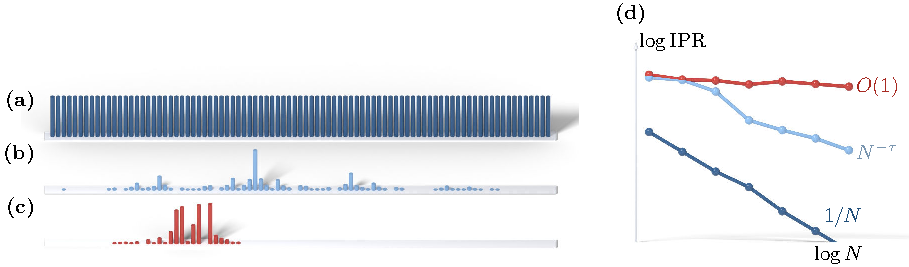
\includegraphics{figures/pdf/s09f06_localization.pdf}
\end{aqmfigure}


\textbf{Fully disordered case.} Now let the on-site potential be genuinely random, of strength $W$,
$H = -t\sum_n (c_n^\dagger c_{n+1} + \text{h.c.}) + \sum_n w_n\, c_n^\dagger c_n$ with $w_n$ drawn
uniformly from $[-W,W]$. At $W=0$ this is an ordinary clean metal with the band structure of the
periodic hopping alone; as $W\to\infty$ every eigenstate collapses onto a single site. In dimension
$d\geq 3$, there is a genuine \textbf{Anderson localization transition} at a finite critical disorder
$W_c$, a true mobility edge separating extended, metallic states from localized ones, exactly the
kind of ``critical point'' described on the slides. Below the transition (or at any energy on the
extended side of a mobility edge) the system conducts; above it, states exist at every energy, so
there is \emph{no spectral gap} in the density of states, but those states cannot carry current, so there
\emph{is} a transport gap: the \textbf{Anderson insulator} is an insulator with no gap in its spectrum at all,
a genuinely unusual state of matter compared to every band or Mott insulator we have met so far in
this course.

\textbf{The special role of one dimension.} In $d=1$ (and, by the scaling theory of localization,
marginally in $d=2$ as well), there is no true metallic phase surviving at any non-zero disorder in
the thermodynamic limit: an arbitrarily small $W>0$ eventually localizes every state. What survives
is a finite localization length $\xi(W)$, which for weak disorder near the band center of the 1D
model scales as $\xi(W) \propto (t/W)^2$, diverging as $W\to 0$. A finite sample shorter than
$\xi(W)$ still looks metallic in practice; only once the sample length exceeds $\xi(W)$ does the
localized, insulating character actually show up in transport. This is the precise sense in which
``weak disorder in 1D'' and ``genuinely metallic'' are never quite the same statement, even though they
can look identical at short length scales.

\begin{notebookbox}{\texttt{session9.ipynb}, ``The impact of disorder in different systems'' (Core), ``Extended and localized states in quasicrystals'' (Challenge), and ``Localization due to random disorder'' (Core)}
Sweep the quasiperiodic modulation strength and separately the random disorder strength $W$, and
compute (9.12) for the resulting eigenstates in each case. Watch $\mathrm{IPR}$ cross over from
$1/N$-like to $O(1)$ behavior as you increase the potential strength, and try to locate, by eye,
where the extended-to-localized crossover happens in each of the two models; compare that to the
critical/mobility-edge language above.
\end{notebookbox}

\section{Closing summary}

\begin{itemize}
\item A perturbation applied to a quantum material and measured elsewhere defines a \textbf{response
  function}; under translational and time-translation symmetry it is most naturally expressed in
  $(q,\omega)$-space (Section 9.1).
\item A classical warm-up already carries the whole session's logic: the sign of the divergence in the
  high-temperature magnetic susceptibility (9.1) predicts, from the disordered phase alone, whether
  the low-temperature order will be ferromagnetic or antiferromagnetic.
\item Linear response theory (9.2)-(9.3) computes the leading effect of any perturbation from the
  unperturbed ground state alone, but breaks down for the orthogonality catastrophe, the Kondo
  effect, and the BCS gap, none of which are perturbatively connected to the unperturbed state.
\item For a Fermi sea, the static and dynamical Lindhard functions (9.4)-(9.5) are built entirely from
  matrix elements between occupied and empty states near the Fermi surface, and diverge whenever a
  nesting vector connects large portions of that surface, signaling an instability (Section 9.4).
\item Summing the interaction to all orders via the random phase approximation (9.6) reveals two
  distinct sources of divergence: electron-hole excitations from $\chi_0$ itself, and collective
  plasmon excitations (9.7) from the RPA denominator.
\item The Stoner criterion (9.8), $U\chi_0(q,0)=1$, recovers session 1 and session 6's magnetism as an
  \emph{instability of the paramagnetic response function}, including the preference for
  antiferromagnetism at a nested (half-filled) Fermi surface, rather than as a mean-field ordered
  ansatz imposed by hand.
\item A local impurity in a metal produces Friedel oscillations (9.9), a power-law-decaying, $2k_F$-periodic
  density modulation that directly images the Fermi surface, the same physics an STM measures via
  quasiparticle interference.
\item A magnetic impurity in a superconductor creates a Yu-Shiba-Rusinov in-gap bound state (9.10),
  whose energy crosses zero at a genuine $S_{\rm tot}=0 \to 1/2$ quantum phase transition; a
  non-magnetic impurity leaves the spectrum essentially untouched.
\item A vacancy in a topological superconductor or Chern insulator produces an in-gap mode purely by
  bulk-boundary correspondence, a diagnostic for topology that a clean, fully gapped bulk spectrum
  alone cannot provide (Section 9.8).
\item Screening of a magnetic impurity in a quantum spin liquid reuses session 8's Abrikosov-fermion
  mean-field construction directly, and inherits the metal-impurity mathematics of Section 9.6: the
  induced spin correlation (9.11) decays as a power law for the gapless spin-1/2 chain and
  exponentially for the gapped spin-1 chain, giving a fully general gapped-versus-gapless diagnostic
  from impurity response alone.
\item Many impurities at once can break translational symmetry throughout the whole system, giving rise
  to Anderson localization: a genuine mobility edge in $d\geq3$, diagnosed by the inverse
  participation ratio (9.12), and a spectral-gap-free but transport-gapped Anderson insulator; in
  one dimension, arbitrarily weak disorder localizes every state, with a diverging localization
  length as the disorder strength goes to zero (Section 9.10).
\end{itemize}

Every session so far has gone in the same direction: start from a Hamiltonian, and compute what it
predicts, whether an observable, a response function, or a ground state. Session 10 turns that
arrow around. Having spent this whole course computing observables from Hamiltonians, next time we
ask the inverse question: given only observed data, can we infer the Hamiltonian that produced it,
and machine learning turns out to be exactly the right tool for making that question precise.
